% Intended LaTeX compiler: pdflatex
\documentclass[11pt]{article}
\usepackage[utf8]{inputenc}
\usepackage[T1]{fontenc}
\usepackage{graphicx}
\usepackage{longtable}
\usepackage{wrapfig}
\usepackage{rotating}
\usepackage[normalem]{ulem}
\usepackage{amsmath}
\usepackage{amssymb}
\usepackage{capt-of}
\usepackage{hyperref}
\author{Construção de compiladores I}
\date{}
\title{Análise LL(1)}
\hypersetup{
 pdfauthor={Construção de compiladores I},
 pdftitle={Análise LL(1)},
 pdfkeywords={},
 pdfsubject={},
 pdfcreator={Emacs 28.2 (Org mode 9.7)}, 
 pdflang={English}}
\begin{document}

\maketitle
\section*{Objetivos}
\label{sec:org8905e4e}

\subsection*{Objetivos}
\label{sec:orga9fffec}

\begin{itemize}
\item Apresentar o algoritmo para construção de tabelas LL(1).

\item Apresentar o algoritmo de análise sintática preditiva.
\end{itemize}
\subsection*{Objetivos}
\label{sec:orgd0856f9}

\begin{itemize}
\item Apresentar uma implementação Haskell do algoritmo.
\end{itemize}
\section*{Gramáticas LL(1)}
\label{sec:org72f3795}

\subsection*{Gramáticas LL(1)}
\label{sec:org8d5e732}

\begin{itemize}
\item Na última aula, definimos os conjuntos first e follow.

\item Usaremos esses conjuntos para definir gramáticas LL(1).
\end{itemize}
\subsection*{Gramáticas LL(1)}
\label{sec:org252a2d5}

\begin{itemize}
\item Para isso, vamos definir o conceito de \(first^{+}\):
\end{itemize}

\begin{array}{l}
first^{+}(A\to\alpha) = first(\alpha)\:\:\:\lambda\not\in first(\alpha)\\
first^{+}(A\to\alpha) = first(\alpha)\cup follow(A)\:\:\:\lambda\in first(\alpha)\\
\end{array}
\subsection*{Gramáticas LL(1)}
\label{sec:org030e80a}

\begin{itemize}
\item Dizemos que uma gramática é LL(1) se:
\end{itemize}

\begin{array}{l}
\forall 1 \leq i, j \leq n, i \neq j \to \\ first^{+}(A\to\alpha_i)\cap first^{+}(A\to\alpha_j) = \emptyset\\
\end{array}
\subsection*{Gramáticas LL(1)}
\label{sec:org159acad}

\begin{itemize}
\item Gramáticas LL(1) admitem analisadores sem retrocesso.

\item Veremos como tal analisador pode ser contruído.
\end{itemize}
\section*{Análise preditiva}
\label{sec:org5737eda}

\subsection*{Análise preditiva}
\label{sec:org0ee2e06}

\begin{itemize}
\item Determina a produção da gramática a ser usada com base no próximo
token da entrada.
\end{itemize}
\subsection*{Análise preditiva}
\label{sec:org64ae369}

\begin{itemize}
\item Analisadores preditivos utilizam uma tabela para decidir qual
regra será utilizada.

\item Tabela construída utilizando os conjuntos first e follow.
\end{itemize}
\subsection*{Análise preditiva}
\label{sec:org862ddf9}

\begin{itemize}
\item Tabela indexada por \(V\) e símbolos de \(\Sigma\) mais o marcador de final de entrada.

\item O símbolo \$ marca o final da entrada.
\end{itemize}
\subsection*{Análise preditiva}
\label{sec:org91f1f7e}

\begin{itemize}
\item Tabela armazena produções da gramática.

\item Entrada \(M[A,a]\) armazena a regra a ser utilizada se \(a\in first(\alpha)\).
\end{itemize}
\section*{Construção da tabela}
\label{sec:org45bc98d}

\subsection*{Construção da tabela}
\label{sec:orgc4bd454}

\begin{itemize}
\item Dada uma gramática \(G\), calcule os conjuntos first e follow de cada não terminal de \(G\).

\item Para cada regra \(A \to \alpha\) da gramática, faça os seguintes passos:
\end{itemize}
\subsection*{Construção da tabela}
\label{sec:org7bab92e}

\begin{itemize}
\item Para cada \(a\in first(A)\), inclua \(A \to \alpha\) em \(M[A,a]\).

\item Se \(\lambda\in first(\alpha)\), inclua \(A\to \alpha\) em \(M[A,b]\) para cada \(b\in follow(A)\).
\end{itemize}
\subsection*{Construção da tabela}
\label{sec:org16c6ca8}

\begin{itemize}
\item Se \(\lambda\in first(\alpha)\) e \$ \(\in follow(A)\), coloque \(A \to \alpha \in\) M[A,\$].
\end{itemize}
\subsection*{Construção da tabela}
\label{sec:orgc7da156}

\begin{itemize}
\item Gramática de exemplo
\end{itemize}

\begin{array}{lcl}
E  & \to & TE'\\
E' & \to & \textbf{+} TE'\,|\, \lambda\\
T  & \to & FT'\\
T' & \to & \textbf{*}FT'\,|\,\lambda\\
F  & \to & \textbf{(}E\textbf{)}\,|\,\textbf{id}\\
\end{array}
\subsection*{Construção da tabela}
\label{sec:orge28653e}

\begin{itemize}
\item first(F) = first (T) = first(E) = \(\{(, id\}\).

\item first(E') = \(\{+,\lambda\}\).

\item first(T') = \(\{*,\lambda\}\).
\end{itemize}
\subsection*{Construção da tabela}
\label{sec:orgd713dbe}

\begin{itemize}
\item follow(E) = follow(E') = \{),\$\}.

\item follow(T) = follow(T') = \{+,),\$\}.

\item follow(F) = \{+, *, ), \$\}.
\end{itemize}
\subsection*{Construção da tabela}
\label{sec:org7a7bfc4}

\begin{itemize}
\item Produção \(E \to TE'\).
\begin{itemize}
\item first(TE') = first(T) = \{(,id\}.
\item \(M[E,id] = M[E,(] = E \to TE'\).
\end{itemize}
\end{itemize}
\subsection*{Construção da tabela}
\label{sec:orgfb688e3}

\begin{itemize}
\item Produção \(E' \to +TE'\).
\begin{itemize}
\item \(first(+TE') = {+}\).
\item \(M[E',+] = E' \to +TE'\).
\end{itemize}
\end{itemize}
\subsection*{Construção da tabela}
\label{sec:orgfd8f344}

\begin{itemize}
\item Produção \(E' \to \lambda\).
\begin{itemize}
\item \(first(\lambda) = \lambda\).
\item follow(E') = \{),\$\}.
\item M[E',)] = M[E',\$] = \(E'\to\lambda\)
\end{itemize}
\end{itemize}
\subsection*{Construção da tabela}
\label{sec:org6cdf3a1}

\begin{itemize}
\item Produção \(T \to FT'\)
\begin{itemize}
\item \(first(T) = first(FT') = \{(,id\}\).
\item \(M[T,(] = M[T,id] = T \to FT'\).
\end{itemize}
\end{itemize}
\subsection*{Construção da tabela}
\label{sec:org3503fca}

\begin{itemize}
\item Produção \(T' \to *FT'\)
\begin{itemize}
\item \(first(*FT') =\{*\}\).
\item \(M[T',*] = T' \to FT'\).
\end{itemize}
\end{itemize}
\subsection*{Construção da tabela}
\label{sec:org1789816}

\begin{itemize}
\item Produção \(T' \to \lambda\)
\begin{itemize}
\item \(first(\lambda) = \lambda\)
\item follow(T') = \{+,),\$\}.
\item M[T',+] = M[T',)] = M[T',\$] = \(T'\to \lambda\).
\end{itemize}
\end{itemize}
\subsection*{Construção da tabela}
\label{sec:org684156c}

\begin{itemize}
\item Produção \(F \to id\)
\begin{itemize}
\item first(id) = \{id\}
\item M[F,id] = id
\end{itemize}
\end{itemize}
\subsection*{Construção da tabela}
\label{sec:orgbeefd52}

\begin{itemize}
\item Produção \(F \to (E)\)
\begin{itemize}
\item first((E)) = \{(\}
\item \(M[F,(] = F \to (E)\)
\end{itemize}
\end{itemize}
\section*{Implementação em Haskell}
\label{sec:org150d160}

\subsection*{Implementação em Haskell}
\label{sec:org9ba53c8}

\begin{itemize}
\item Definição da tabela
\end{itemize}

\begin{verbatim}
type Table = Map (Nonterminal, Terminal) [Production]
\end{verbatim}
\subsection*{Implementação em Haskell}
\label{sec:org768f747}

\begin{itemize}
\item Construção da tabela
\end{itemize}

\begin{verbatim}
buildTable :: Grammar -> Table
buildTable g = foldr step Map.empty (productions g)
  where
    firstG = first g
    followG = follow g
    insertTable p s tbl
       = Map.insertWith union (leftHand p, s) [p] tbl 
\end{verbatim}
\subsection*{Implementação em Haskell}
\label{sec:org484719b}

\begin{itemize}
\item Construção da tabela
\end{itemize}

\begin{verbatim}
step p tbl
   = let 
       firstM = Map.fromList firstG
       lhs = leftHand p
       rhs = rightHand p
       firstP = firstForWord rhs firstM
       followP = maybe [] id (lookup lhs followG)
       tbl1 = foldr (insertTable p) tbl [x | x <- firstP, x /= Lambda]
       tbl2 = if Lambda `elem` firstP
              then foldr (insertTable p) tbl1 followP
              else tbl1
     in if Lambda `elem` firstP &&
           Dollar `elem` followP
        then insertTable p Dollar tbl2
        else tbl2
\end{verbatim}
\section*{Análise preditiva}
\label{sec:org353258d}

\subsection*{Análise preditiva}
\label{sec:org6787e49}

\begin{itemize}
\item O algoritmo utiliza:
\begin{itemize}
\item Tabela
\item Pilha
\end{itemize}
\end{itemize}
\subsection*{Análise preditiva}
\label{sec:orgc6240f9}

\begin{itemize}
\item Estrutura do analisador
\end{itemize}

\begin{center}
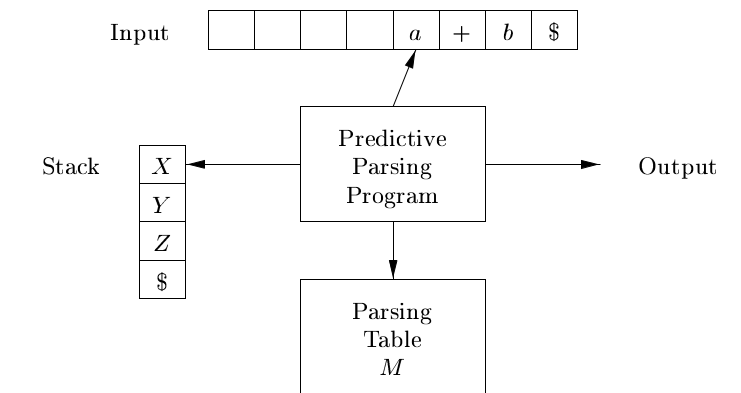
\includegraphics[width=.9\linewidth]{./imgs/predictive.png}
\end{center}
\subsection*{Análise preditiva}
\label{sec:org4b24c8c}

\begin{itemize}
\item Inicialização
\begin{itemize}
\item Entrada w\$
\item Pilha: Símbolo de partida no topo, \$ no fundo.
\end{itemize}
\end{itemize}
\subsection*{Análise preditiva}
\label{sec:orgffb9ea0}

\begin{itemize}
\item Seja \(X\) o símbolo de topo da pilha.
\item Seja \(a\) o primeiro token da entrada.
\item Se \(X = a\), desempilhe \(X\) e obtenha próximo token.
\end{itemize}
\subsection*{Análise preditiva}
\label{sec:org3bd87db}

\begin{itemize}
\item Se \(X\) é um não terminal, seja \(r = M[X,a]\).

\item Se \(r\) é erro, pare.

\item Se \(r = X \to Y_1 ... Y_k\)
\begin{itemize}
\item Desempilhe \(X\).
\item Empilhe \(Y_k ... Y_1\).
\end{itemize}
\end{itemize}
\subsection*{Análise preditiva}
\label{sec:org292f1b5}

\begin{itemize}
\item Vamos considerar a gramática
\end{itemize}

\begin{array}{lcl}
E  & \to & TE'\\
E' & \to & \textbf{+} TE'\,|\, \lambda\\
T  & \to & FT'\\
T' & \to & \textbf{*}FT'\,|\,\lambda\\
F  & \to & \textbf{(}E\textbf{)}\,|\,\textbf{id}\\
\end{array}
\subsection*{Análise preditiva}
\label{sec:org8104fa6}

\begin{itemize}
\item Vamos considerar a string id + id.
\end{itemize}
\subsection*{Análise preditiva}
\label{sec:org5090e98}

\begin{itemize}
\item Inicialização
\begin{itemize}
\item Entrada: id + id\$
\item Pilha: E\$
\end{itemize}
\end{itemize}
\subsection*{Análise preditiva}
\label{sec:orgbad811f}

\begin{itemize}
\item Temos que:
\begin{itemize}
\item \(X = E\)
\item \(a = id\)
\end{itemize}
\end{itemize}
\subsection*{Análise preditiva}
\label{sec:org6021e1a}

\begin{itemize}
\item Temos que \(M[E,id]= E \to TE'\)
\begin{itemize}
\item Entrada: id+id\$
\item Pilha: TE'\$
\end{itemize}
\end{itemize}
\subsection*{Análise preditiva}
\label{sec:org10623b7}

\begin{itemize}
\item Temos que:
\begin{itemize}
\item \(X = T\)
\item \(a = id\)
\end{itemize}
\end{itemize}
\subsection*{Análise preditiva}
\label{sec:org9f7e5c0}

\begin{itemize}
\item Temos que \(M[T,id] = T\to FT'\)
\begin{itemize}
\item Entrada: id+id\$
\item Pilha: FT'E'\$.
\end{itemize}
\end{itemize}
\subsection*{Análise preditiva}
\label{sec:orge545354}

\begin{itemize}
\item Temos que:
\begin{itemize}
\item \(X = F\)
\item \(a = id\)
\end{itemize}
\end{itemize}
\subsection*{Análise preditiva}
\label{sec:org2e0e302}

\begin{itemize}
\item Temos que \(M[F,id] = F \to id\)
\begin{itemize}
\item Entrada: id + id\$
\item Pilha: idT'E'\$.
\end{itemize}
\end{itemize}
\subsection*{Análise preditiva}
\label{sec:org662595d}

\begin{itemize}
\item Temos que:
\begin{itemize}
\item \(X=id\).
\item \(a = id\).
\end{itemize}
\end{itemize}
\subsection*{Análise preditiva}
\label{sec:org5d91f77}

\begin{itemize}
\item Como \(X = a\), desempilhamos \(X\) e obtemos próximo token.
\begin{itemize}
\item Entrada: +id\$
\item Pilha: T'E'\$.
\end{itemize}
\end{itemize}
\subsection*{Análise preditiva}
\label{sec:org32a237e}

\begin{itemize}
\item Temos que:
\begin{itemize}
\item \(X = T'\).
\item \(a = +\).
\end{itemize}
\end{itemize}
\subsection*{Análise preditiva}
\label{sec:org7e11af7}

\begin{itemize}
\item Temos que \(M[T',+] = T'\to\lambda\).
\begin{itemize}
\item Entrada: +idE
\item Pilha: E'\$.
\end{itemize}
\end{itemize}
\subsection*{Análise preditiva}
\label{sec:orgef40640}

\begin{itemize}
\item Temos que:
\begin{itemize}
\item \(X = E'\).
\item \(a = +\).
\end{itemize}
\end{itemize}
\subsection*{Análise preditiva}
\label{sec:orga570187}

\begin{itemize}
\item Temos que \(M[E',+] = E'\to + TE'\).
\begin{itemize}
\item Entrada: +id\$
\item Pilha: +TE'\$
\end{itemize}
\end{itemize}
\subsection*{Análise preditiva}
\label{sec:org7c89cf4}

\begin{itemize}
\item Temos que
\begin{itemize}
\item \(X = +\)
\item \(a = +\)
\end{itemize}
\end{itemize}
\subsection*{Análise preditiva}
\label{sec:org056550e}

\begin{itemize}
\item Como \(X = a\), desempilhamos \(X\) e obtemos o próximo token.
\begin{itemize}
\item Entrada: id\$.
\item Pilha: TE'\$.
\end{itemize}
\end{itemize}
\subsection*{Análise preditiva}
\label{sec:org04e799d}

\begin{itemize}
\item Temos que
\begin{itemize}
\item \(X = T\)
\item \(a = id\)
\end{itemize}
\end{itemize}
\subsection*{Análise preditiva}
\label{sec:org5c0a91f}

\begin{itemize}
\item Temos que \(M[T,id] = T\to FT'\)
\begin{itemize}
\item Entrada: id\$
\item Pilha: FT'E'\$
\end{itemize}
\end{itemize}
\subsection*{Análise preditiva}
\label{sec:org0a012ef}

\begin{itemize}
\item Temos que
\begin{itemize}
\item \(X = F\)
\item \(a = id\)
\end{itemize}
\end{itemize}
\subsection*{Análise preditiva}
\label{sec:org2c5736e}

\begin{itemize}
\item Temos que \(M[F,id] = F \to id\)
\begin{itemize}
\item Entrada: id\$
\item Pilha: idT'E'\$.
\end{itemize}
\end{itemize}
\subsection*{Análise preditiva}
\label{sec:org6930fa6}

\begin{itemize}
\item Temos que
\begin{itemize}
\item \(X = id\).
\item \(a = id\).
\end{itemize}
\end{itemize}
\subsection*{Análise preditiva}
\label{sec:orga32b94a}

\begin{itemize}
\item Como \(X = a\), desempilhamos \(X\) e obtemos o próximo token.
\begin{itemize}
\item Entrada: \$
\item Pilha: T'E'\$.
\end{itemize}
\end{itemize}
\subsection*{Análise preditiva}
\label{sec:org1486fa9}

\begin{itemize}
\item Temos que:
\begin{itemize}
\item \(X = T'\).
\item a = \$.
\end{itemize}
\end{itemize}
\subsection*{Análise preditiva}
\label{sec:orged92fb8}

\begin{itemize}
\item Temos que M[T',\$] = \(T'\to\lambda\):
\begin{itemize}
\item Entrada: \$
\item Pilha: E'\$
\end{itemize}
\end{itemize}
\subsection*{Análise preditiva}
\label{sec:org5a3d0d8}

\begin{itemize}
\item Temos que:
\begin{itemize}
\item \(X = E'\).
\item a = \$.
\end{itemize}
\end{itemize}
\subsection*{Análise preditiva}
\label{sec:org4bc21da}

\begin{itemize}
\item Temos que M[E',\$] = \(E'\to\lambda\):
\begin{itemize}
\item Entrada: \$
\item Pilha: \$
\end{itemize}
\end{itemize}
\subsection*{Análise preditiva}
\label{sec:orgc09f32f}

\begin{itemize}
\item Temos que:
\begin{itemize}
\item X = \$
\item a = \$
\end{itemize}
\end{itemize}
\subsection*{Análise preditiva}
\label{sec:org583e310}

\begin{itemize}
\item como \(X = a\), desempilhamos \(X\) e como não há próximo token o algoritmo encerra com sucesso.
\end{itemize}
\section*{Implementação em Haskell}
\label{sec:org0b3d798}

\subsection*{Implementação em Haskell}
\label{sec:org25fb91d}

\begin{itemize}
\item Definição do estado do algoritmo
\end{itemize}

\begin{verbatim}
data Pred
  = Pred {
      stack :: [Symbol]
    , input :: String
    , table :: Table
    }
\end{verbatim}
\subsection*{Implementação em Haskell}
\label{sec:org7d87b40}

\begin{itemize}
\item Inicialização
\end{itemize}

\begin{verbatim}
initial :: Grammar -> String -> Pred
initial g s
  = Pred stk (s ++ "$") (buildTable g)
    where
      stk = [Var (start g), Symb Dollar]
\end{verbatim}
\subsection*{Implementação em Haskell}
\label{sec:orgbd583fc}

\begin{itemize}
\item Implementação da análise preditiva
\end{itemize}

\begin{verbatim}
predictiveM :: Lexer -> PredictiveM ()
predictiveM plex
  = do
      v <- emptyStack
      if v then return ()
      else do
          r <- nextToken plex
          a <- top
          when (isTerminal a && a /= (Symb r)) (throwError $ expecting a r)
          when (isTerminal a && a == (Symb r)) (pop >> consumeToken plex)
          when (isNonterminal a) $ do
            let nt' = nonTerminal a
            v <- pop
            p <- lookupTable nt' r
            when (isNothing p) (throwError "Parsing table error!")
            let p' = fromJust p
            push (rightHand p')
          predictiveM plex
\end{verbatim}
\section*{Concluindo}
\label{sec:org252ca2e}

\subsection*{Concluindo}
\label{sec:orga92c964}

\begin{itemize}
\item Nesta aula apresentamos o algoritmo de análise sintática preditiva.

\item Apresentamos uma implementação deste algoritmo em Haskell
\end{itemize}
\subsection*{Concluindo}
\label{sec:org05a5d5d}

\begin{itemize}
\item Próxima aula: análise sintática ascendente.
\end{itemize}
\section*{Exercícios}
\label{sec:orgf258545}

\subsection*{Exercícios}
\label{sec:org13fd151}

\begin{itemize}
\item Estenda o algoritmo de análise preditiva para que este verifique se a
gramática fornecida é ou não LL(1).
\end{itemize}
\end{document}
